\documentclass[11pt,a4paper]{article}

% تنظیمات حاشیه صفحه
\usepackage{geometry}
\geometry{top=2cm, bottom=2cm, left=1.5cm, right=1.5cm}

% بسته‌های مورد نیاز برای ستون‌بندی و گرافیک
\usepackage{multicol}
\usepackage{graphicx}
\usepackage{xcolor}
\usepackage{framed}
\usepackage{caption}
\usepackage{listings}
\usepackage{pgfplots}
\usetikzlibrary{calc,angles,quotes}
\usepackage{booktabs}
\usepackage[titletoc]{appendix} 
\usepackage{xepersian}
\usepackage{lmodern} 
\usepackage{amsmath}
\usepackage{amssymb}
\usepackage{fancyhdr}

\settextfont[Scale=1.1]{XB Niloofar}
\setlatintextfont[Scale=1.0]{Times New Roman}
\setdigitfont[Scale=1.1]{XB Niloofar}

\begin{document}
% ----------------- بخش عنوان -----------------
\begin{center}
    {\Huge \textbf{هایزنبرگ، عدم قطعیت و انقلاب کوانتومی}}\\[1.5em]
    
    {\Large \textit{در ۳۲ سالگی، ورنر هایزنبرگ یکی از جوان‌ترین دانشمندانی بود که جایزه نوبل را دریافت کرد. جاه‌طلبی و رقابت‌جویی شدید، الهام‌بخش او در فرمول‌بندی یکی از شناخته‌شده‌ترین اصول علم شد.}}\\[1.5em]
    
    {\large از \lr{David C. Cassidy}}
\end{center}

\vspace{1.5em}

\setlength{\columnsep}{0.8cm}

\begin{multicols}{3}
\noindent از میان دستاوردهای متعدد علم در قرن بیستم، شاید بنیادی‌ترین آن‌ها مکانیک کوانتومی باشد. این علم که توسط گروه کوچکی از فیزیکدانان بسیار بااستعداد اروپایی ابداع شد، علم اتم مستلزم تحولات عمیق و بحث‌برانگیزی در درک ما از طبیعت است. ماده می‌تواند موج یا ذره باشد (بسته به نحوه مشاهده آن‌ها) و علت و معلول دیگر ارتباط نزدیکی با هم ندارند. این تفسیر از مکانیک کوانتومی -- دستورالعمل‌هایی برای چگونگی و زمان استفاده از آن و آنچه در مورد دنیای فیزیکی به ما می‌گوید -- در سال ۱۹۲۷ در کپنهاگ توسعه یافت. به دلیل ترویج آن توسط بنیانگذارانش و موفقیت حیرت‌انگیز متخصصانش، تفسیر کپنهاگی تا دهه ۱۹۳۰ به برتری دست یافت که امروزه نیز از آن برخوردار است. اما یک تفسیر فقط یک تفسیر است. ریشه‌ها، دفاع و پذیرش آن از جنبه‌های مهمی می‌تواند محصول شرایط تاریخی و ترجیح شخصی و همچنین اعتبار علمی باشد.

نقشی که ویژگی‌های انسانی در علم ایفا می‌کنند شاید به بهترین وجه توسط یکی از مخترعان اصلی و فعال‌ترین حامیان تفسیر کپنهاگی نشان داده شود، یعنی ورنر کارل هایزنبرگ. در فوریه ۱۹۲۷ بود که دستیار فوق‌دکتری ۲۵ ساله نیلز بور شناخته‌شده‌ترین سهم خود را در فیزیک و عنصر کلیدی تفسیر کپنهاگی را فرمول‌بندی کرد: اصل عدم قطعیت یا عدم تعین. مانند تفسیر کپنهاگی، این را می‌توان نتیجه جستجو برای وسیله‌ای سازگار جهت پیوند دادن دنیای روزمره آزمایشگاه با دنیای عجیب و جدید ریزاتم دانست.

\vspace{1em}
\noindent\fbox{
\parbox{0.9\linewidth}{
\footnotesize
\textbf{دیوید سی. کاسیدی} دانشیار دانشگاه هافسترا و یکی از ویراستاران همکار در \textit{مجموعه مقالات آلبرت اینشتین} است. او دکترای خود را در تاریخ علم از دانشگاه پردو در سال ۱۹۷۶ دریافت کرد. اقامت شش ساله او در آلمان، ابتدا به عنوان عضو الکساندر فون هومبولت در دانشگاه اشتوتگارت و سپس به عنوان استادیار در دانشگاه رگنسبورگ، او را قادر ساخت تا تحقیقات گسترده‌ای در مورد هایزنبرگ و تاریخ علم آلمان انجام دهد. کتاب او با عنوان \textit{عدم قطعیت: زندگی و علم ورنر هایزنبرگ} سال گذشته توسط W. H. Freeman and Company منتشر شد.
}
}
\vspace{1em}

به طور خلاصه، اصل عدم قطعیت بیان می‌کند که اندازه‌گیری همزمان دو متغیر اصطلاحاً مزدوج، مانند موقعیت و تکانه یک ذره متحرک، مستلزم محدودیت ضروری در دقت است. هرچه اندازه‌گیری موقعیت دقیق‌تر باشد، اندازه‌گیری تکانه نامشخص‌تر خواهد بود و بالعکس. در شدیدترین حالت، دقت مطلق یک متغیر شامل بی‌دقتی مطلق در مورد دیگری است.

این عدم تعین تقصیر آزمایشگر نیست: این یک پیامد بنیادی معادلات کوانتومی و ویژگی هر آزمایش کوانتومی است. علاوه بر این، هایزنبرگ اعلام کرد، تا زمانی که مکانیک کوانتومی معتبر است، بر اصل عدم قطعیت هرگز غلبه نخواهد شد. برای اولین بار از زمان انقلاب علمی، یک فیزیکدان پیشرو محدودیتی در درک علمی را اعلام کرده بود.

در کنار ایده‌های بزرگانی چون بور و ماکس بورن، اصل عدم قطعیت هایزنبرگ سیستم منطقاً بسته تفسیر کپنهاگی را تشکیل داد که هایزنبرگ و بورن قبل از نشست فیزیکدانان کوانتومی پیشرو جهان در اکتبر ۱۹۲۷ آن را کامل و غیرقابل‌برگشت اعلام کردند. آن نشست، پنجمین کنگره از کنگره‌های معروف سُلوِی (Solvay) در مورد فیزیک بنیادی که در بروکسل برگزار شد، و تنها چند هفته پس از انتصاب هایزنبرگ به کرسی فیزیک نظری در دانشگاه لایپزیگ دنبال شد. او تنها با ۲۵ سال سن، جوان‌ترین استاد تمام آلمان بود.

\vspace{1em}
\noindent جوانی مفرط هایزنبرگ در زمان مهم‌ترین کارش نشان‌دهنده ویژگی مهمی است که بر این و تمام تحقیقات اولیه او تأثیر گذاشت: انگیزه تقریباً سیری‌ناپذیر او برای موفقیت تحصیلی و متمایز شدن به عنوان بهترین در هر کاری که انجام می‌داد. جای تعجب نیست که بخش زیادی از این تمایل را می‌توان در میراث خانوادگی او ردیابی کرد.

خانواده هایزنبرگ خانواده‌ای بسیار بافرهنگ و جاه‌طلب بودند که در حال باز کردن راه خود به طبقه متوسط رو به بالای جامعه آلمان بودند. اتحاد آلمان در اواخر قرن نوزدهم تحت رهبری اتو فون بیسمارک و رشد اقتصادی قدرتمند پس از آن، نیاز شدیدی به دیوان‌سالاران، دیپلمات‌ها، قضات، وکلا و مدیران ایجاد کرده بود. در نتیجه، دانشگاه‌ها و مدارس کشور به طور چشمگیری اهمیت یافتند. اعتبار و پاداش‌های مادی دانشگاهیان و دانش‌آموزان موفق آنها نیز همینطور بود.

هم پدر ورنر، آگوست، و هم پدربزرگ مادری‌اش، نیکولاس وِکلین، از ریشه‌های محقر از طریق پیشرفت تحصیلی به بالاترین سطوح بورژوازی عالی آلمان رسیده بودند. وکلین در یک دبیرستان (گیمنازیوم) معروف در مونیخ مدیریت داشت و در آگوست ۱۹۱۰ استاد لغت‌شناسی بیزانسی در دانشگاه مونیخ شد. هر دو مرد نیز در جایگاه‌های جدید خود ازدواج کردند.

درست از زمان تولد ورنر در سال ۱۹۰۱، بزرگان او مصمم بودند که او نیز از طریق دانش‌پژوهی به موقعیت اجتماعی بالایی دست یابد. آگوست با این باور که رقابت باعث شکوفایی موفقیت تحصیلی می‌شود، رقابت شدیدی بین ورنر و برادر بزرگترش اروین ایجاد کرد. در طول سال‌ها دو پسر اغلب به شدت با هم می‌جنگیدند، رقابت آنها یک روز به یک نبرد خونین ختم شد که در آن با صندلی‌های چوبی یکدیگر را کتک زدند. در بزرگسالی، هر یک راه خود را رفتند -- اروین به برلین نقل مکان کرد و شیمیدان شد -- و به استثنای گردهمایی‌های گاه‌به‌گاه خانوادگی، تماس کمی با هم داشتند.

جاه‌طلبی ورنر برای رسیدن به اوج به ویژه در دوره بین ژوئیه ۱۹۲۵، زمانی که او و همکارانش بورن و پاسکوال جردن توصیف ریاضی مکانیک کوانتومی را توسعه دادند، و فوریه ۱۹۲۷، زمانی که او روابط عدم قطعیت را فرمول‌بندی کرد، مشهود است. آنچه تأثیر چنین انگیزه‌ای را در این دوران بسیار قابل توجه کرد، تلاقی دو پیشرفت بود.

اول، چندین کرسی فیزیک نظری به طور ناگهانی در اروپای مرکزی آلمانی‌زبان خالی شد. این موقعیت‌ها به معنای فرصت عالی برای یک آکادمیک جاه‌طلب مانند هایزنبرگ بود که قبلاً صلاحیت (\textit{Habilitation}) دریافت کرده بود، یعنی برای کرسی تدریس دانشگاهی در دانشگاه گوتینگن واجد شرایط شده بود.

دوم، و شاید مهم‌تر از همه، ظهور یک توصیف ریاضی جدید و رقیب برای مکانیک کوانتومی بود. هایزنبرگ و همکارانش در سال ۱۹۲۵ فرمالیسمی برای مکانیک کوانتومی توسعه داده بودند که مبتنی بر ریاضیات انتزاعی حساب ماتریسی بود. برای نویسندگان آن، این «مکانیک ماتریسی» ترجیح آنها را برای تکیه صرف بر مشاهدات آزمایشگاهی در بر می‌گرفت. آنها به ملزوماتی مانند وجود پرش‌های کوانتومی و ناپیوستگی‌ها درون اتم‌ها پایبند بودند و ایده مدل‌های اتمی \textit{anschaulich} یا قابل تصویرسازی را رد کردند.

اروین شرودینگر، فیزیکدان ۳۹ ساله وینی که در آن زمان در زوریخ کار می‌کرد، از جهتی کاملاً متفاوت و با اهدافی کاملاً متفاوت به معماهای فیزیک اتمی نزدیک شد. در مجموعه‌ای از مقالات منتشر شده در نیمه اول سال ۱۹۲۶، شرودینگر یک معادله موج کوانتومی را بر اساس فرضیه‌ای که توسط کاندیدای دکترای فرانسوی، لویی دوبروی مطرح شده بود، ارائه کرد. این ایده که مورد توجه مساعد اینشتین قرار گرفت، این بود که تمام مواد در حال حرکت می‌توانند به عنوان موج در نظر گرفته شوند. شرودینگر از این مفهوم استفاده کرد تا ادعا کند که الکترون «امواج ماده»، حالت‌های هماهنگ ارتعاش را درون اتم‌ها ایجاد می‌کند. این حالت‌ها جایگزین حالت‌های اتمی ثابت نظریه ماتریسی می‌شوند؛ پرش‌های کوانتومی ناپیوسته به جای آن، گذارهای پیوسته از یک حالت هارمونیک به حالت دیگر هستند. اگر درست بود، شرودینگر به تازگی اصول مکانیک ماتریسی هایزنبرگ را بی‌ربط ساخته بود.

بیشتر فیزیکدانان با کمال میل از رویکرد آشناتر شرودینگر استقبال کردند و درباره تفسیر او از آن کمتر گفتند. این وضعیت در ماه مه ۱۹۲۶، زمانی که شرودینگر اثباتی منتشر کرد مبنی بر اینکه دو فرمالیسم رقیب، در واقع، از نظر ریاضی معادل هستند، ناگهان تغییر کرد. هایزنبرگ و همکاران ماتریسی او فوراً به دفاع از هدف خود برخاستند و با لحنی که در هر دو طرف به طور فزاینده‌ای احساسی می‌شد.

شرودینگر به بهبود اوضاع کمکی نکرد. در مقاله هم‌ارزی خود، او نه برای قدردانی برابر از دو طرح متضاد، بلکه برای برتری طرح خود استدلال کرد. در یک پاورقی معروف در مقاله خود، او بیان کرد: «هیچ رابطه ژنتیکی [بین کار هایزنبرگ و من] برای من شناخته شده نیست. البته من از نظریه او مطلع بودم، اما از روش‌های جبر استعلایی که به نظرم دشوار می‌آمد و عدم وجود \textit{Anschaulichkeit} [قابلیت تصویرسازی]، احساس دلسردی، تا نگویم دفع‌شدگی، کردم.»

هایزنبرگ نیز در نامه‌ای به همکار نزدیک خود ولفگانگ پاولی به همان شکل پاسخ داد: «هرچه بیشتر درباره بخش فیزیکی نظریه شرودینگر فکر می‌کنم، آن را دفع‌کننده‌تر می‌یابم.... آنچه شرودینگر در مورد قابلیت تصویرسازی نظریه‌اش می‌نویسد «احتمالاً کاملاً درست نیست» [بازتابی از بور]، به عبارت دیگر این \textit{Mist} [مزخرف] است.» تنها مزیت روش شرودینگر، همانطور که علناً گفت، این بود که امکان محاسبه ساده احتمالات گذار اتمی، یا احتمالات پرش‌های کوانتومی را برای قرار دادن در ماتریس‌های مکانیک کوانتومی فراهم می‌کرد. پاولی موافق بود.

\vspace{1em}

\noindent نگاهی دقیق‌تر به زمان‌بندی این اظهارات نشان می‌دهد که این هم‌ارزی نبود که باعث درگیری شد (پاولی آن را یک ماه قبل به صورت خصوصی و بدون هیاهو ثابت کرده بود) بلکه آنچه هر طرف از آن استنباط کرد بود. هایزنبرگ و مکتب ماتریس تمام دوران حرفه‌ای خود را صرف مبارزه با خواصی از طبیعت کرده بودند که معتقد بودند وجود دارد و در مکانیک ماتریسی آن‌ها تجسم یافته است. آن‌ها آینده خود را روی این رویکرد شرط‌بندی کرده بودند. شرودینگر اعتبار خود را در از بین بردن ناپیوستگی‌های به ظاهر غیرمنطقی و پرش‌های کوانتومی از طریق احیای فیزیک پیوسته، علی و حرکات موجی منطقی به خطر انداخته بود. هیچ یک از طرفین حاضر نبود برتری -- یا پیامد احتمالی آن یعنی تسلط حرفه‌ای -- را به دیگری واگذار کند. ماهیت و مسیر آینده مکانیک کوانتومی ناگهان مورد مناقشه قرار گرفت.
این اختلاف، جاه‌طلبی‌های شغلی هایزنبرگ را بیشتر تشدید کرد. تنها چند هفته قبل از انتشار اثبات

\end{multicols}

\vspace*{\fill}
\begin{center}
    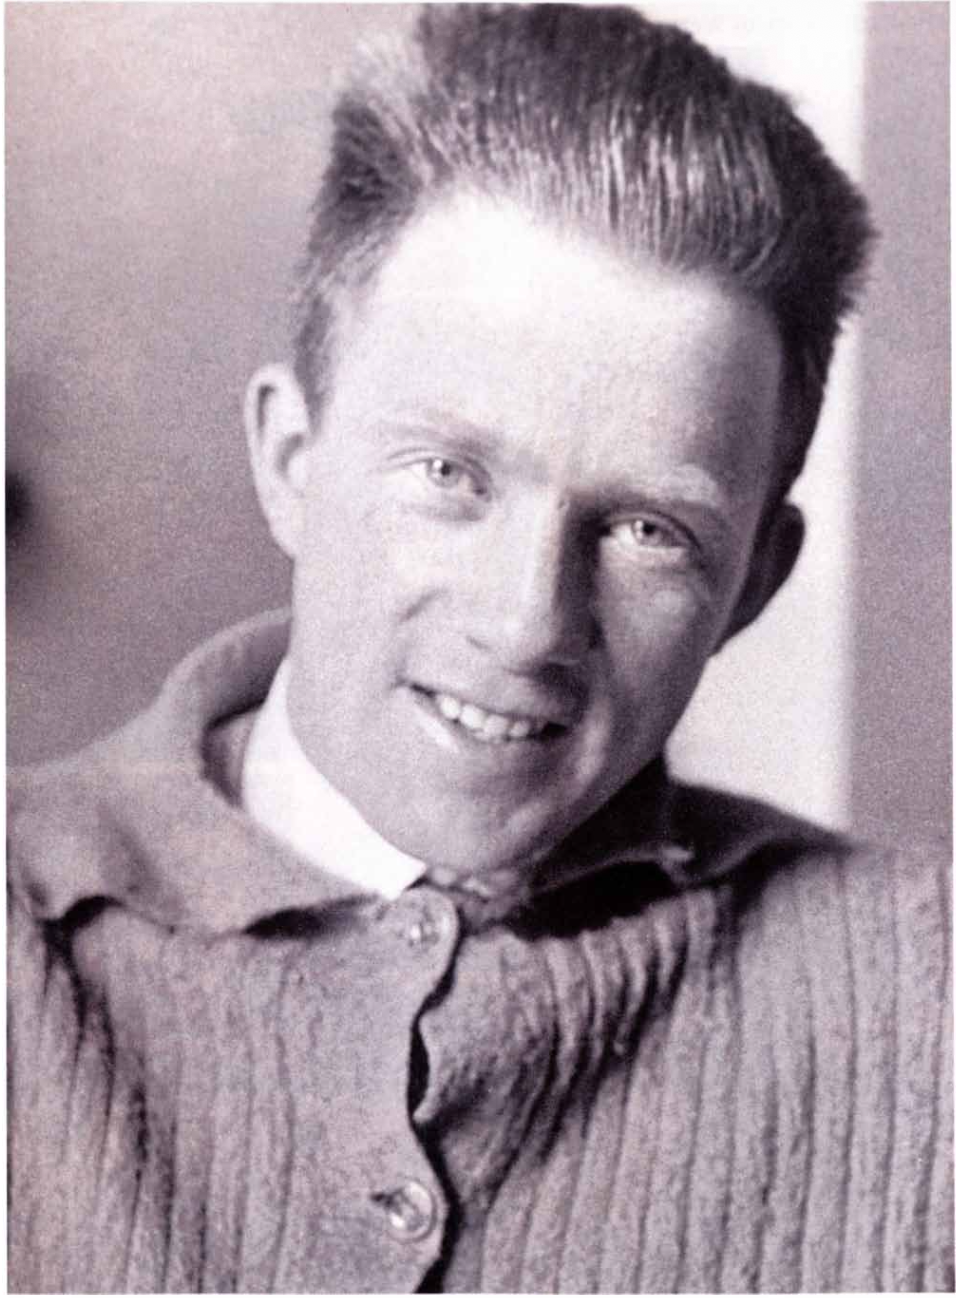
\includegraphics[width=\textwidth,height=0.9\textheight, keepaspectratio]{young he}
    
    \textbf{ورنر هایزنبرگ مهم‌ترین سهم‌های خود را در دههٔ بیست‌سالگی‌اش به فیزیک ارائه کرد. این عکس حدود سال ۱۹۲۴ در دانشگاه گوتینگن گرفته شده است؛ جایی که او سخنرانی‌ای را ارائه داد که او را برای احراز کرسی دانشگاهی واجد شرایط کرد.}
\end{center}
\vspace*{\fill}

\newpage

\vspace*{\fill}
\begin{center}
    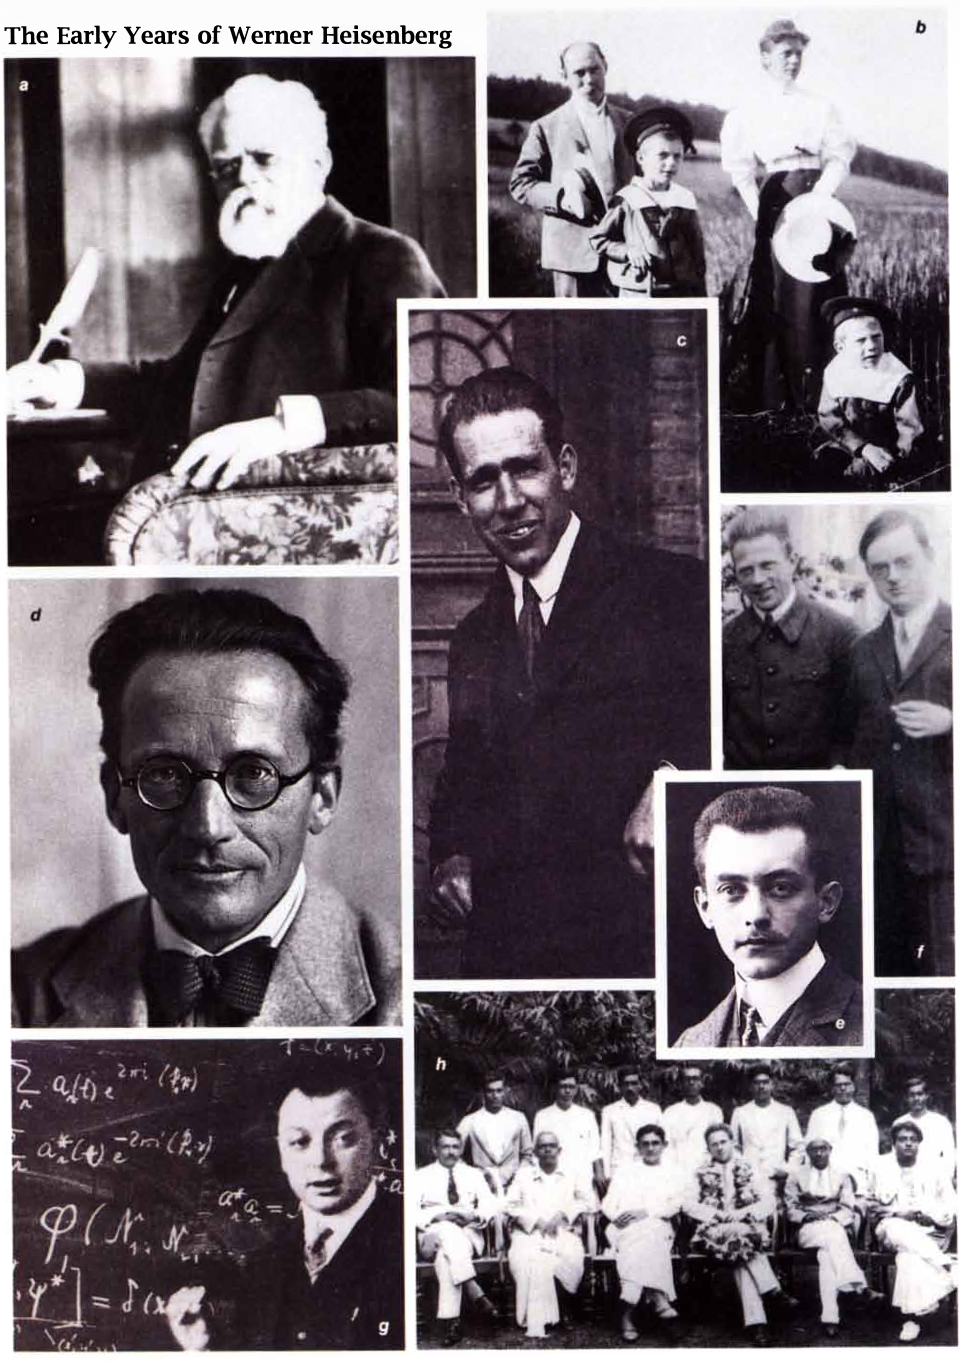
\includegraphics[width=\textwidth,height=0.9\textheight, keepaspectratio]{other}
    \\ \textbf{سال‌های آغازین ورنر هایزنبرگ}
\end{center}
\vspace*{\fill}

\newpage

\begin{multicols}{3}

 هم‌ارزی توسط شرودینگر، هایزنبرگ استادی دانشگاه لایپزیگ را به نفع دستیاری با بور در کپنهاگ رد کرده بود. پدربزرگ ناباور ورنر، وکلین، درست در زمانی که مقاله هم‌ارزی شرودینگر ظاهر شد، شتابان به کپنهاگ رفت تا در تلاشی نوه خود را از پذیرش آن پست منصرف کند. فشارهای مجدد وکلین و چالش شرودینگر بر پایه‌های فیزیک ماتریسی، تلاش‌های هایزنبرگ را برای تولید اثری با چنان کیفیتی که پذیرش حرفه‌ای گسترده‌ای به دست آورد و در نهایت او را در کرسی خالی دیگری قرار دهد، دوچندان کرد.

اما دست کم سه رویداد در سال ۱۹۲۶، شکاف فکری عمیق بین ایده‌های او و دیدگاه شرودینگر را به او گوشزد کرد. اولین مورد، سخنرانی‌های شرودینگر درباره فیزیک جدیدش در مونیخ در پایان ژوئیه بود. در آنجا هایزنبرگ جوان از میان حضار شلوغ استدلال کرد که نظریه شرودینگر چندین پدیده را توضیح نمی‌دهد. او در متقاعد کردن کسی موفق نشد و کنفرانس را با ناامیدی ترک کرد. سپس، در طول کنفرانس پاییزی دانشمندان و پزشکان آلمانی، هایزنبرگ شاهد حمایت قاطع -- و از نظر او، اشتباه -- از دیدگاه‌های شرودینگر بود.

در نهایت، بحث شدید اما در نهایت بی‌نتیجه بین بور و شرودینگر در کپنهاگ در اکتبر ۱۹۲۶ وجود داشت. نتیجه بحث، اذعان به این بود که هیچ تفسیر درستی از هیچ‌یک از فرمالیسم‌های کوانتومی کاملاً قابل قبول نیست. با این حال، هر طرفی که بتواند چنین تفسیری پیدا کند، قادر خواهد بود، همانطور که گفته می‌شود بور بیان کرد، «آرزوهایش» را برای فیزیک آینده محقق سازد.

با این انگیزه‌های مختلف -- شخصی، حرفه‌ای و علمی -- تا فوریه ۱۹۲۷ هایزنبرگ معتقد بود که ناگهان به تفسیر مورد نیاز دست یافته است: اصل عدم قطعیت. مسیر فکری او به سوی آن ایده در اواخر ۱۹۲۶ و اوایل ۱۹۲۷ در تحقیقات نزدیک‌ترین همکارانش، به ویژه جردن و پل آ. م. دیراک نهفته بود، که با هم «نظریه تبدیل»، ادغام مکانیک موجی و مکانیک ماتریسی را فرمول‌بندی کردند.

\end{multicols}

\vspace{1.5em}
\noindent\fbox{
\parbox{\linewidth}{
\small
\textbf{تأثیرات بر زندگی هایزنبرگ} با پدربزرگش، نیکولاس وکلین (\textbf{a}) و پدرش، آگوست، که با همسرش آنا، و پسرانش، اروین (ایستاده) و ورنر (\textbf{b}) نشان داده شده است، آغاز شد. هر دو مرد میل به موفقیت تحصیلی را در پسران پرورش دادند. هایزنبرگ زیر نظر نیلز بور (\textbf{c}) تحصیل کرد، که بعداً تفسیر کپنهاگی را با او توسعه داد. یکی از اولین رقبای هایزنبرگ اروین شرودینگر (\textbf{d}) بود که فرمالیسم موجی او مکانیک ماتریسی را که هایزنبرگ در سال ۱۹۲۵ با ماکس بورن (\textbf{e}) و پاسکوال جردن (\textbf{f}، راست) توسعه داد، به چالش کشید. ولفگانگ پاولی (\textbf{g}) محرک اصلی در کمک به هایزنبرگ برای توسعه اصل عدم قطعیت در سال ۱۹۲۷ بود. در سال ۱۹۲۹ هایزنبرگ برای گسترش "روح کپنهاگ" یک تور سخنرانی جهانی را آغاز کرد و به ایالات متحده، ژاپن، چین و در نهایت هند (\textbf{h}) رسید.
}
}
\begin{figure}[ht!]
    \centering
    \fbox{
        \parbox{0.95\linewidth}{
            \centering
            \vspace{0.5em}
            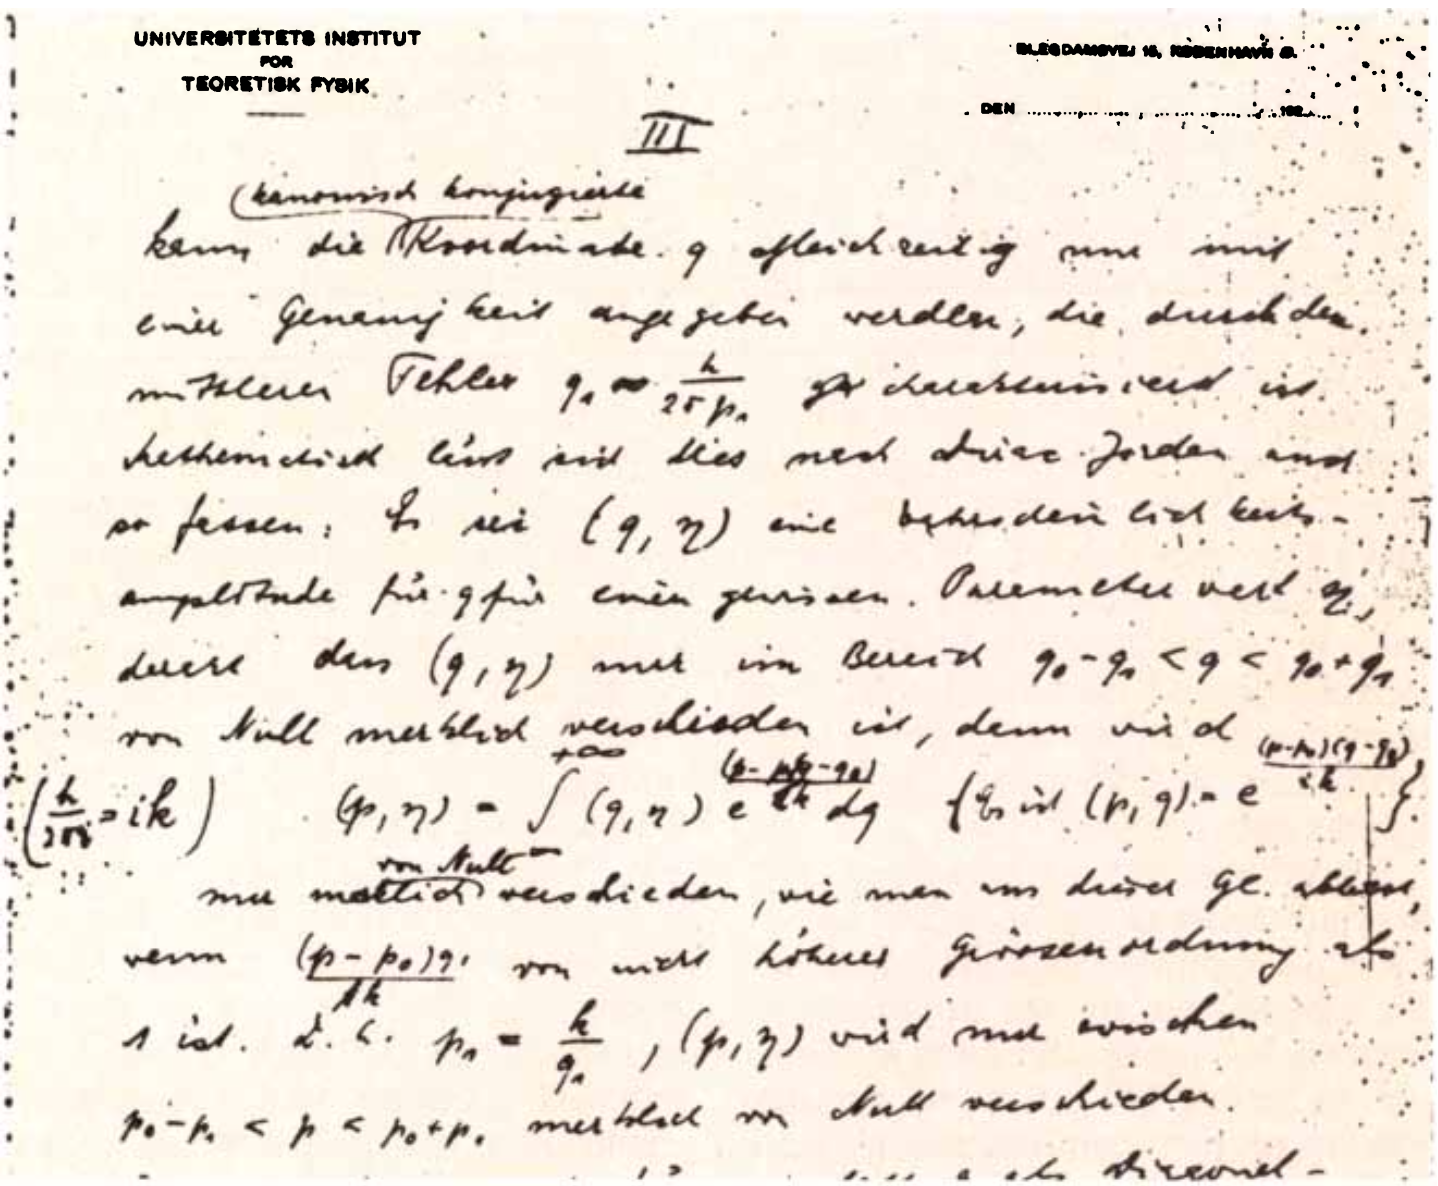
\includegraphics[width=0.6\textwidth]{Heisenberg Note} 
            \vspace{1em}
            
            \parbox{0.95\linewidth}{
                \small
                \textbf{نامه‌ای که توسط هایزنبرگ} به ولفگانگ پاولی نوشته شد، روابط عدم قطعیت را برای $p$ و $q$ استخراج کرد، جایی که $p_1 = \sqrt{2} \Delta p$ و $q_1 = \sqrt{2} \Delta q$. این گزیده، بخشی از یک نامه ۱۴ صفحه‌ای، مبنای مقاله اصل عدم قطعیت هایزنبرگ بود.
            }
            \vspace{0.5em}
        }
    }
\end{figure}

\vspace{1.5em}

\setlength{\columnsep}{0.8cm}

\begin{multicols}{3}
و ریاضیات ماتریسی. بنابراین هدف هایزنبرگ و متحدانش یافتن راهی غیرقابل‌انکار برای گنجاندن ناپیوستگی در فرمالیسم دیراک و جردن بود.

انگیزه اصلی برای این تفسیر جدید از جانب پاولی بود. او در نامه‌اش به تاریخ ۱۹ اکتبر ۱۹۲۶، که در آن به هایزنبرگ در مورد کرسی خالی در لایپزیگ اطلاع داد، حالت‌های اتمی ثابت را در مطالعه پیشین بورن درباره امواج الکترون آزاد اعمال کرد. او متوجه شد که باید متغیرهای پیوسته برای تکانه $p$ و موقعیت $q$ یک الکترون اتمی انتخاب شوند، اما رفتار کوانتومی آنها یک «نقطه تاریک» را نشان می‌داد: «باید فرض کرد که متغیرهای $p$ کنترل می‌شوند، و متغیرهای $q$ کنترل نمی‌شوند. یعنی فرد می‌تواند فقط احتمالات تغییرات معین متغیرهای $p$ را برای شرایط اولیه معین محاسبه کند و از میانگین تمام مقادیر ممکن متغیرهای $q$ استفاده کند.» پاولی نوشت: «بنابراین، نمی‌توان از یک «مسیر» مشخص برای ذره صحبت کرد، و نه می‌توان به طور همزمان در مورد مقدار $p$ و مقدار $q$ پرس و جو کرد.»

هایزنبرگ پاسخ داد که از نامه پاولی و نقطه تاریک آن «بسیار هیجان‌زده» است، موضوعی که هایزنبرگ طی ماه‌های بعد مرتباً روی آن فکر می‌کرد. اشتیاق هایزنبرگ در نامه‌ای ۱۴ صفحه‌ای به پاولی در ۲۳ فوریه ۱۹۲۷ به اوج خود رسید. در آن، او تقریباً تمام ویژگی‌های اساسی مقاله‌ای را که دقیقاً یک ماه بعد با عنوان «درباره محتوای \textit{anschaulich} [قابل تصویرسازی] سینماتیک و مکانیک کوانتومی» ارسال شد، ارائه کرد: مقاله اصل عدم قطعیت هایزنبرگ.

هایزنبرگ با استخراج روابط عدم قطعیت هم از ریاضیات و هم از آزمایش‌های فکری، توافق بین این دو را به عنوان اثباتی بر اعتبار جهانی عدم قطعیت در نظر گرفت. استدلال ریاضی با یک تابع موج آغاز شد که به صورت یک منحنی زنگوله‌ای، یا از نظر ریاضی، یک توزیع احتمال گاوسی، برای متغیر $q$ در نظر گرفته شده بود. خطای دانستن مقدار دقیق $q$ (که انحراف معیار نامیده می‌شود) دلتا $q$ است که به صورت $\Delta q$ نوشته می‌شود. با استفاده از فرمالیسمی که توسط دیراک و جردن توسعه یافته بود، هایزنبرگ توزیع گاوسی را به متغیر مزدوج $p$ تبدیل کرد.

\vspace{0.5em}
\noindent با انجام این کار، او دریافت که به عنوان یک پیامد ریاضی، انحرافات معیار این دو توزیع -- یعنی عدم دقت در مقادیر $q$ و $p$ -- با یکدیگر رابطه عکس دارند. این تقابل می‌تواند گسترش یافته و با این رابطه بیان شود:
$$ \Delta p \cdot \Delta q \ge \frac{h}{4\pi} $$
که در آن $h$ ثابت پلانک است. سپس او نشان داد که این نتیجه صرفاً انتزاعی نیست، بلکه با هر آزمایش قابل تصوری که شامل اندازه‌گیری همزمان جفت متغیرهای مزدوج، مانند موقعیت و تکانه یا انرژی و زمان باشد، کاملاً سازگار است.

با این حال، سازگاری با آزمایش به چندین نوآوری که هایزنبرگ به منظور گنجاندن ناپیوستگی و ذرات معرفی کرد، متکی بود. یکی از این موارد، بازتعریف کلمه آلمانی \textit{anschaulich} در عنوان مقاله‌اش بود که به معنای «فیزیکی» یا دارای معنای تجربی به جای قابل تصویرسازی یا تصویری باشد. این تغییر به منظور مقابله با انتقاد شرودینگر مبنی بر اینکه فیزیک ذرات ناپیوسته اساساً غیرمنطقی و \textit{unanschaulich} است، در نظر گرفته شده بود. این امر با نوآوری دوم ارتباط نزدیکی داشت: بازتعریف مفاهیم کلاسیکی مانند موقعیت، سرعت و مسیر یک ذره اتمی بر اساس عملیات تجربی مورد استفاده برای اندازه‌گیری آن‌ها، شکلی از عملیات‌گرایی. تنها آنچه فیزیکدان می‌تواند اندازه‌گیری کند معنای واقعی دارد و این اندازه‌گیری‌ها همیشه روابط عدم قطعیت را نشان می‌دهند.

برای هایزنبرگ جوان، اصل عدم قطعیت نقطه اوج و تکمیل انقلاب کوانتومی بود، انقلابی که تعهدات او به پایه‌هایی که خودش به پایه‌گذاری آن‌ها کمک کرده بود را در بر می‌گرفت. و گویی برای خاموش کردن هرگونه اعتراضی به این دیدگاه، او مقاله منتشر شده خود را با چندین ادعا که بسیار فراتر از ریاضیات و آزمایش فکری بود، به پایان رساند. او اعلام کرد که با نظریه تبدیل دیراک-جردن، فرمالیسم کوانتومی کامل و غیرقابل تغییر است؛ روابط عدم قطعیت درست و غیرقابل انکار هستند، زیرا آن‌ها نتیجه مستقیم این فرمالیسم می‌باشند. بنابراین، تمام مشاهدات تجربی قبلی و آینده از پدیده‌های اتمی تحت این تفسیر قرار می‌گیرند.

علاوه بر این، او استدلال کرد که اگرچه فیزیک کوانتومی حاوی یک عنصر آماری اساسی است، اما این عنصر ویژگی خود طبیعت نیست. این عنصر به دلیل اختلال ناشی از تلاش فیزیکدان برای مشاهده طبیعت وارد می‌شود. در نهایت، او اولین بیانیه صریح خود را در مورد یکی از عمیق‌ترین پیامدهای عدم قطعیت -- چالشی برای علیت -- ارائه داد.

اصل علیت ایجاب می‌کند که قبل از هر معلولی، یک علت منحصر به فرد وجود داشته باشد. این ایده برای بیش از یک قرن به عنوان یک فرض اساسی تقریباً در هر شکلی از تحقیقات منطقی عمل کرده بود. ریاضیدان فرانسوی لاپلاس شاید ساده‌ترین تعریف علیت را در کاربرد آن در مکانیک نیوتنی ارائه کرده است: اگر موقعیت و تکانه یک ذره در یک لحظه مشخص با دقت شناخته شود، آنگاه با آگاهی از تمام نیروهای وارد بر ذره، حرکت آن برای تمام زمان‌های آینده به طور کامل توسط معادلات مکانیکی تعیین می‌شود.

هایزنبرگ ادعا کرد که اصل عدم قطعیت این را رد می‌کند: «در فرمول‌بندی دقیق قانون علی -- اگر حال را بدانیم، می‌توانیم آینده را محاسبه کنیم - این نتیجه‌گیری نیست که اشتباه است، بلکه پیش‌فرض اشتباه است.» مقادیر اولیه تکانه و موقعیت را نمی‌توان به طور همزمان با دقت مطلق اندازه‌گیری کرد. بنابراین، فرد تنها می‌تواند محدوده‌ای از احتمالات را برای موقعیت و تکانه ذره در هر زمان آینده محاسبه کند. تنها یک احتمال از حرکت واقعی ذره نتیجه خواهد شد. ارتباط علی بین حال و آینده از بین می‌رود، و قوانین و پیش‌بینی‌های مکانیک کوانتومی طبیعتاً صرفاً احتمالاتی یا آماری می‌شوند.

مقاله اصل عدم قطعیت هایزنبرگ تقریباً از هر نظر عمیق و گسترده بود. علاوه بر برآورده کردن دقیق اهدافش، مقاله هایزنبرگ از نظر شخصیتی نیز بازتاب او بود. زمانی که استادش، بور، او را با خطایی در استدلال مواجه کرد، هایزنبرگ سرسختانه از موضع خود در نبردی دفاع کرد که در بهار ۱۹۲۷ به آنچه هایزنبرگ «سوءتفاهمات شخصی فاحش» نامید، تنزل یافت. این خطا شامل اتکای بیش از حد هایزنبرگ به ناپیوستگی و ویژگی‌های ذره‌ای کوانتوم‌های نور در یکی از آزمایش‌های فکری اساسی‌اش، یعنی اصطلاحاً میکروسکوپ پرتو گاما بود [کادر زیر را ببینید].

\vspace{0.5em}
\noindent بور، که در تعطیلات اسکی بود، بازگشت و متوجه شد که مقاله هایزنبرگ در حال حاضر در مرحله پیش‌نویس است. با ارسال مقاله به اینشتین به درخواست هایزنبرگ، بور به طور خصوصی به اینشتین شکایت کرد که کل رویکرد هایزنبرگ بسیار محدود بود و میکروسکوپ پرتو گامای او کاملاً اشتباه بود، اگرچه نتیجه درست بود. برای بور، روابط عدم قطعیت صرفاً از فرمالیسم، بازتعریف مفاهیم اساسی و برتری ناپیوستگی و ذرات بر امواج پیوسته ناشی نمی‌شد. دوگانگی موج-ذره و، در میکروسکوپ پرتو گاما، پراکندگی امواج نور توسط الکترون به داخل عدسی میکروسکوپ نیز بسیار مهم بودند.

تصاویر موج و ذره توصیفاتی «مکمل» یکدیگر هستند، که متقابلاً ناسازگار اما در عین حال مشترکاً برای توصیف ضروری می‌باشند. بور استدلال کرد که آزمایشگر باید انتخاب کند که آزمایش را با تصویر موج یا تصویر ذره تجزیه و تحلیل کند. بهایی که فرد برای چنین جانب‌داری می‌پردازد، محدودیتی در آنچه می‌توان از آزمایش آموخت ایجاد می‌کند، و این محدودیت توسط روابط عدم قطعیت نشان داده می‌شود. بنابراین برای بور، استدلال هایزنبرگ تنها مورد خاصی از چیزی بود که بور اکنون آن را مکمل بودن می‌نامید.

هایزنبرگ به شدت مخالفت کرد. او با پافشاری بر استفاده اولیه از ذرات و ناپیوستگی، مطلقاً پیشنهاد بور مبنی بر پس گرفتن مقاله‌اش را، که در این بین برای چاپ فرستاده بود، رد کرد. هایزنبرگ نمی‌توانست استفاده گسترده از امواج یا مفاهیم مکانیک موجی را تحمل کند، و همچنین نمی‌توانست از انتشار سهم مهم خود در بحث تفسیر صرف‌نظر کند. نبرد متعاقب آن با بور آنقدر شدید شد که بنا بر گزارش‌ها ورنر در طول یک جلسه به گریه افتاد و حتی موفق شد بورِ معمولاً خونسرد را با چند اظهار نظر تند آزرده کند.

\end{multicols}
 
\newpage
\begin{framed}
\begin{center}
    {\Large \textbf{آزمایش فکری میکروسکوپ پرتو گاما}}
\end{center}

\begin{multicols}{2}

\noindent برای نشان دادن اصل عدم قطعیت، هایزنبرگ یک آزمایش فکری ارائه داد. او با استفاده از میکروسکوپی که وضوح آن بالا بود زیرا برای روشنایی به پرتوهای گاما متکی بود، سعی کرد نشان دهد که موقعیت و تکانه الکترون از اصل عدم قطعیت پیروی می‌کنند. اگرچه هایزنبرگ به نتایج درستی دست یافت، بور اشاره کرد که آزمایش اولیه دو اصل اساسی را نادیده گرفته است: قدرت تفکیک میکروسکوپ و دوگانگی موج-ذره.

در نسخه صحیح اجرا شده، یک الکترون آزاد مستقیماً زیر عدسی شیئی میکروسکوپ قرار دارد. عدسی دایره‌ای مخروطی با زاویه $2\Theta$ از الکترون تشکیل می‌دهد. سپس الکترون توسط یک پرتو گاما که از سمت چپ حرکت می‌کند روشن می‌شود. بر اساس یکی از اصول اپتیک موج، میکروسکوپ می‌تواند اجسام را تا اندازه $\Delta x$ تفکیک کند، که به $\Theta$ و به طول موج نور، $\lambda$، توسط این عبارت مرتبط است:
$$ \Delta x = \frac{\lambda}{\sin \Theta} $$

در لحظه‌ای که نور به داخل شیئی میکروسکوپ پراکنده می‌شود، الکترون به سمت راست پس‌زنی می‌کند. پس از برخورد، پرتو گامای مشاهده شده می‌تواند به هر زاویه‌ای درون مخروط $2\Theta$ پراکنده شده باشد. در شدیدترین حالت پراکندگی به لبه جلویی (راست) عدسی، تکانه در جهت $x$ به این صورت خواهد بود:
$$ p'_x + \frac{h}{\lambda'} \sin \Theta, $$

\columnbreak

\noindent که در آن $p'_x$ تکانه الکترون در جهت $x$ است، $\lambda'$ طول موج پرتو گامای منحرف شده است، $h$ ثابت پلانک است (که فرکانس فوتون را به انرژی آن مرتبط می‌کند) و $\frac{h}{\lambda'}$ تکانه کل فوتون پرتو گاما است، همانطور که توسط اصول کوانتومی تعریف شده است. در انتهای دیگر، پرتو گاما به سمت عقب پراکنده می‌شود، و فقط به لبه چپ عدسی برخورد می‌کند. در این حالت، تکانه کل در راستای $x$ به این صورت است:
$$ p''_x - \frac{h}{\lambda''} \sin \Theta. $$

تکانه نهایی در راستای $x$ در هر دو حالت باید برابر با تکانه اولیه باشد؛ بنابراین،
$$ p'_x + \frac{h}{\lambda'} \sin \Theta = p''_x - \frac{h}{\lambda''} \sin \Theta. $$

اگر $\Theta$ کوچک باشد، آنگاه $\lambda' \sim \lambda'' \sim \lambda$، و
$$ p''_x - p'_x = \Delta p_x \sim \frac{2h}{\lambda} \sin \Theta. $$

از آنجا که $\Delta x = \frac{\lambda}{\sin \Theta}$، یک رابطه متقابل بین حداقل عدم قطعیت‌ها در موقعیت‌های اندازه‌گیری شده الکترون در امتداد محور $x$ و تکانه آن در جهت $x$ وجود دارد:
$$ \Delta p_x \sim \frac{h}{\Delta x}. $$

برای بیش از حداقل عدم قطعیت، ممکن است یک نابرابری معرفی شود،
$$ \Delta p_x \cdot \Delta x \ge h, $$
که تقریباً همان رابطه عدم قطعیت هایزنبرگ است.

\end{multicols}

\vspace{0.5em}
\begin{center}
     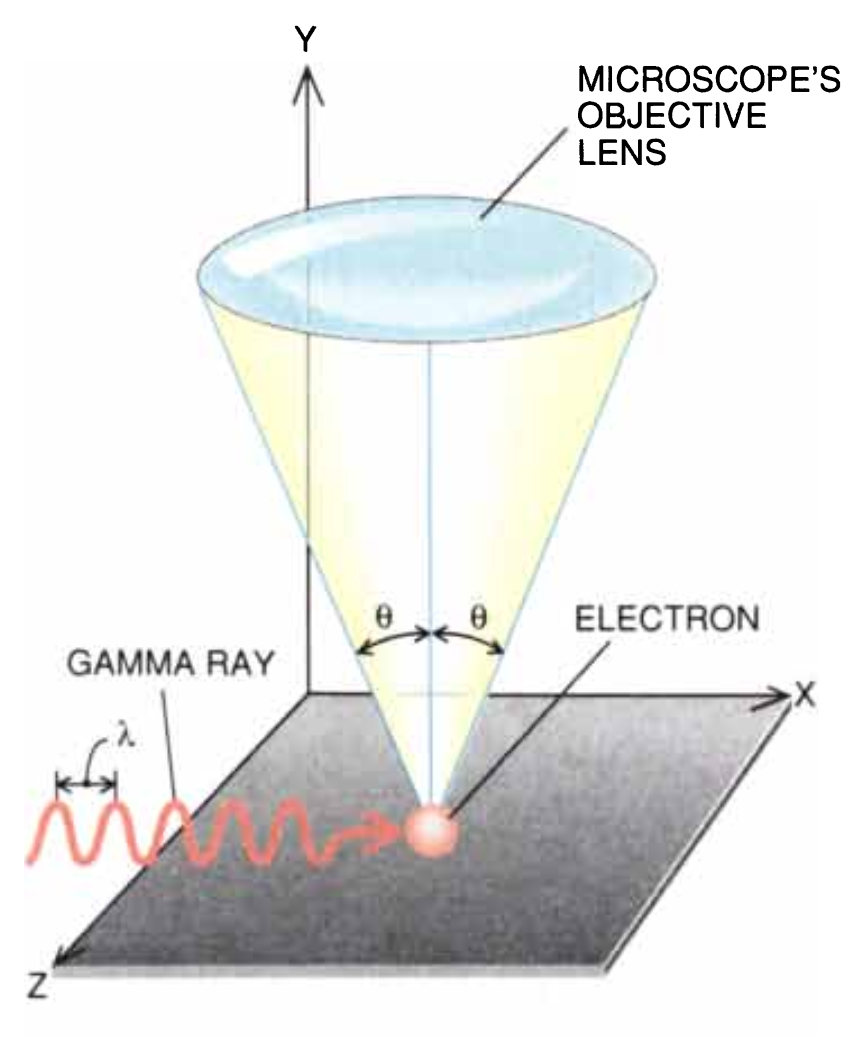
\includegraphics[width=0.3\textwidth]{gamma} 
\end{center}

\end{framed}
\begin{figure}[h]
    \centering
    \fbox{\parbox{0.8\textwidth}{
        \centering
        \vspace{1cm}
         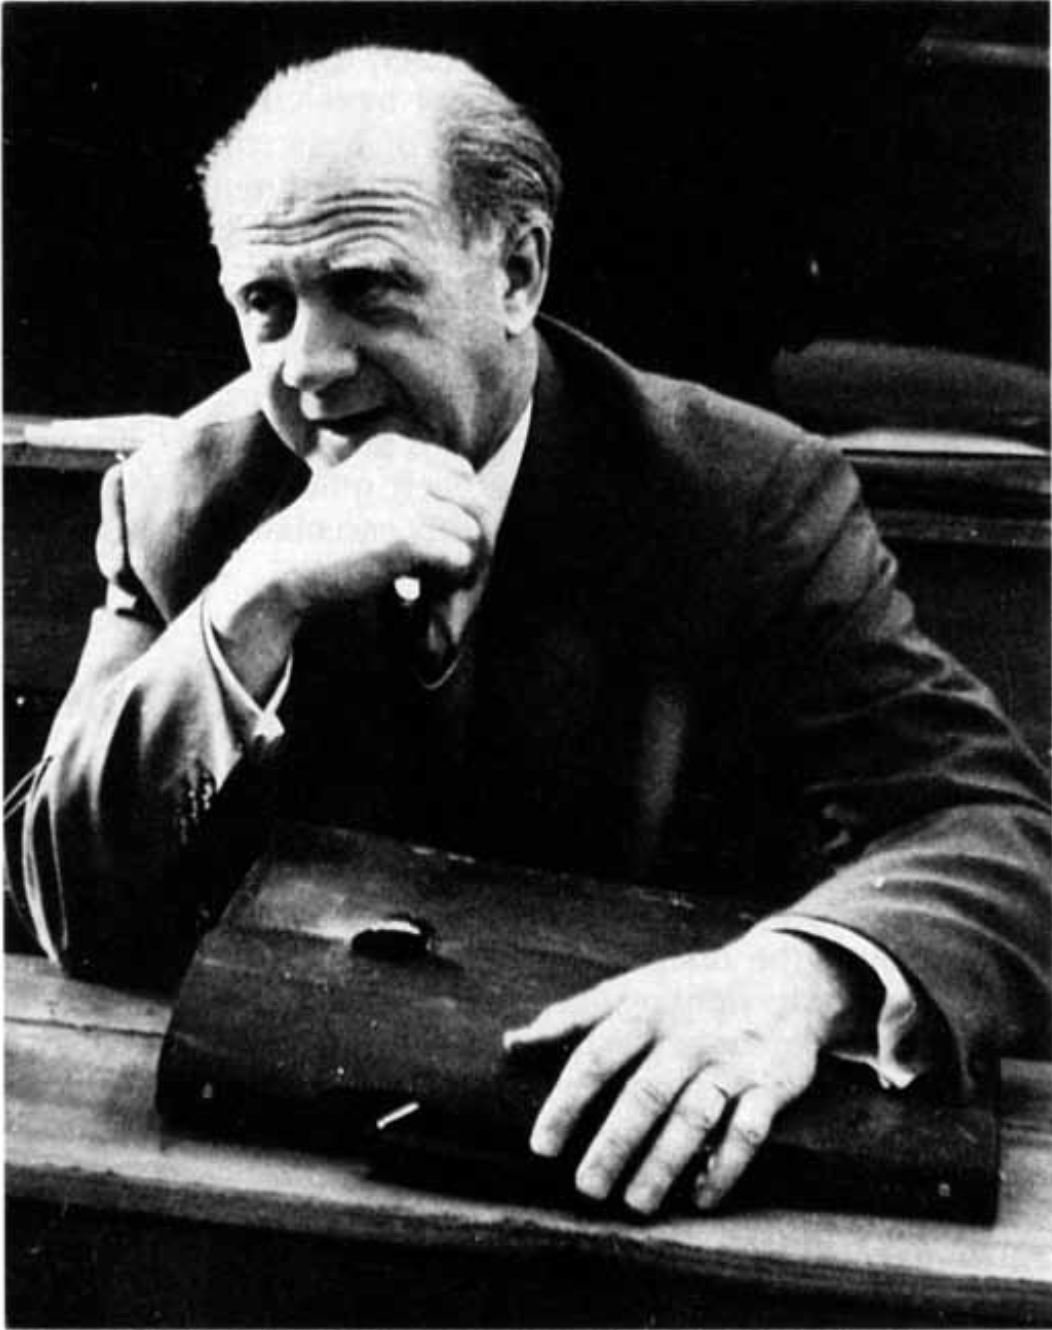
\includegraphics[width=0.6\textwidth]{old he} 
        \vspace{1cm}
    }}
    
    \vspace{0.5em}
    \parbox{0.8\textwidth}{
        \small
        \textbf{هایزنبرگ در ۶۵ سالگی} به دانشگاه لایپزیگ بازگشت تا سخنرانی‌هایی به عنوان مهمان ارائه دهد. او چند سال بعد بیمار شد و در سال ۱۹۷۶ بر اثر سرطان درگذشت.
    }
\end{figure}
\vspace{1em}

% ----------------- شروع متن سه‌ستونی -----------------
\setlength{\columnsep}{0.8cm}
\begin{multicols}{3}

چیزهای زیادی برای این جوان ۲۵ ساله در میان بود: بینش‌های جدیدش، برنامه‌های آکادمیک او و شاید حتی تمایل او برای برابری فکری با مربیانش. مقاله او بدون تجدید نظر در ماه می در یک مجله پیشرو فیزیک آلمانی ظاهر شد، اما حاوی یک پی‌نوشت کوتاه بود که به خطای میکروسکوپ اعتراف می‌کرد و خوانندگان را از برخی اصول اولیه استدلال بور آگاه می‌ساخت.

حدود چهار ماه بعد، هایزنبرگ اشک‌هایش را پاک کرد و لحن خود را کاملاً تغییر داد: به نظر می‌رسید او از انتقاد بور سپاسگزار است. پس از آنکه بور اولین ارائه خود از اصل مکملیت را برای مخاطبانی که در دریاچه کومو در ایتالیا در سپتامبر ۱۹۲۷ گرد هم آمده بودند انجام داد، هایزنبرگ که پیش از این به عدم قطعیت بسیار مطمئن بود، اولین قدردانی سخاوتمندانه خود را به بور تقدیم کرد. در نسخه منتشر شده از بحث پس از مقاله کوموی بور، هایزنبرگ از او به خاطر روشن کردن عدم قطعیت «در تمام جزئیات» و بیان آنچه به عنوان تفسیر کپنهاگی شناخته شد، تشکر کرد.

تغییر رویه هایزنبرگ ممکن است با تحقق جاه‌طلبی‌اش آغاز شده باشد. زیرا در همان ماهِ کنفرانس کومو، هایزنبرگ از دعوت قریب‌الوقوع خود برای کرسی لایپزیگ مطلع شده بود. آن هدف سرانجام محقق شده بود.

با فروکش کردن تمایل هایزنبرگ برای تأکید بر توانایی‌ها و مشارکت‌هایش در مکانیک کوانتومی، تمایل دیگری پدیدار شد که اکنون شامل بور نیز می‌شد: نیاز به ایجاد یک برنامه تحقیقاتی دائمی و درجه یک در لایپزیگ بر اساس این فیزیک. علاوه بر تقویت عدم قطعیت که به خوبی استدلال نشده بود، توضیحات بور نقطه اتکایی برای پیروان این دانشمند دانمارکی فراهم کرد که مانند هایزنبرگ، مشتاق یک فیزیکِ کامل بودند تا آن را از کرسی‌های تازه به دست آمده خود ترویج دهند و در مقالات خود از آن بهره‌برداری کنند. هایزنبرگ و سایر شاگردان بور دیگر وفاداری خود را به برنامه‌ها و اکتشافات فردی، مکانیک ماتریسی یا عدم قطعیت معطوف نمی‌کردند، بلکه به «روح کپنهاگی» وفادار بودند.

هایزنبرگ و دیگران موفق شدند پذیرش تفسیر خود را تضمین کنند، علی‌رغم اعتراضات ماندگار رهبرانی مانند اینشتین و شرودینگر. در طول نیم دهه پس از نشست کومو و، بعدتر، کنگره سولوِی، هایزنبرگ و مؤسسه‌اش نظریه‌های کوانتومی عمده‌ای در مورد بلورهای حالت جامد، ساختار مولکولی، پراکندگی تابش توسط هسته‌ها و ساختار نوترون-پروتون هسته‌ها تولید کردند. آنها به همراه سایر نظریه‌پردازان، گام‌های عظیمی به سوی یک نظریه کوانتومی نسبیتی میدان‌ها برداشتند و پایه‌های تحقیقات فیزیک انرژی بالا را بنا نهادند.

چنین موفقیت‌هایی طبیعتاً بسیاری از بهترین دانشجویان را به مؤسساتی مانند مؤسسه هایزنبرگ جذب کرد. این دانشجویان، که با دکترین کپنهاگ پرورش یافته بودند، نسل جدید و مسلطی از فیزیکدانان را تشکیل دادند که در پی به قدرت رسیدن هیتلر در دهه ۱۹۳۰ و پراکنده شدن در سراسر جهان، این ایده‌ها را با خود به همراه بردند.

هایزنبرگ و دیگر کپنهاگی‌ها زمان کمی را برای رساندن دکترین خود به کسانی که به مؤسسات اروپایی سفر نمی‌کردند، هدر دادند. به طور خاص، هایزنبرگ ایالات متحده را میدان حاصلخیزی برای تبلیغ یافت. در طی یک تور جهانی با دیراک در سال ۱۹۲۹، هایزنبرگ سخنرانی‌های بسیار تأثیرگذاری را در مورد دکترین کپنهاگ در دانشگاه شیکاگو ارائه کرد. هایزنبرگ در پیشگفتار سخنرانی‌های خود نوشت: «به نظر من، هدف این کتاب زمانی برآورده می‌شود که بتواند تا حدودی به گسترش آن \textit{روح کپنهاگی نظریه کوانتومی} (Kopenhagener Geist der Quantentheorie) کمک کند... که تمام توسعه فیزیک اتمی مدرن را هدایت کرده است.»

مروج این \textit{روح} به لایپزیگ بازگشت در حالی که تعهدات علمی قبلی او اکنون به طور گسترده توسط حرفه‌ای پذیرفته شده بود که موقعیت‌های برجسته‌ای را هم از نظر نهادی و هم از نظر علمی به او اعطا می‌کرد. در سال ۱۹۳۳، این حرفه با اعطای جایزه نوبل به همراه شرودینگر و دیراک، برترین تقدیر را از کار او به عمل آورد.

اگرچه امروزه از هایزنبرگ به درستی به عنوان یکی از بزرگترین فیزیکدانان دوران مدرن تجلیل می‌شود، اما او به دلیل بسیاری از اقداماتش پس از به قدرت رسیدن هیتلر مورد انتقاد نیز قرار گرفته است. هایزنبرگ هرگز به حزب نازی نپیوست، اما مناصب برجسته آکادمیک داشت و به سخنگوی فرهنگ آلمان در سرزمین‌های اشغالی تبدیل شد. او با رد مکرر پیشنهادات مهاجرت، ریاست تلاش‌های تحقیقاتی اصلی روی شکافت اورانیوم را برای رایش سوم بر عهده گرفت. پس از جنگ، او توضیحات مختلفی برای اقدامات خود ارائه داد که شهرت او را در خارج از کشور بیش از پیش خدشه‌دار کرد. کنار هم قرار گرفتن گیج‌کننده چنین رفتار سؤال‌برانگیزی با فیزیک درخشان، بازتاب مخمصه‌های بزرگتر دانشمند و علم در طول یک قرن پرآشوب و گاه وحشیانه است. هایزنبرگ، فرزند وفادار آلمان، که نگاهی چنین عمیق به طبیعت داشت، درک و پذیرش اینکه کشورش تا چه حد به طرز غم‌انگیزی گمراه شده است را دشوار یافت. او در سال ۱۹۷۶ بر اثر سرطان کلیه و کیسه صفرا در خانه خود در مونیخ درگذشت.

\vspace{1em}
\noindent\fbox{
\parbox{0.95\linewidth}{
\begin{center}
    \small \textbf{برای مطالعه بیشتر}
\end{center}
\vspace{0.2em}
\begin{latin}
\footnotesize
\noindent \textsc{The Shaky Game: Einstein, Realism and the Quantum Theory.} Arthur Fine. University of Chicago Press, 1986.\\
\vspace{0.3em}

\noindent \textsc{Schrödinger: Life and Thought.} Walter J. Moore. Cambridge University Press, 1989.\\
\vspace{0.3em}

\noindent \textsc{Niels Bohr's Times: In Physics, Philosophy and Polity.} Abraham Pais. Oxford University Press, 1991.\\
\vspace{0.3em}

\noindent \textsc{Uncertainty: The Life and Science of Werner Heisenberg.} David C. Cassidy. W. H. Freeman and Company, 1991.
\end{latin}
}
}

\end{multicols}

\end{document}